\chapter{Misc stuff -- to be moved elsewhere}
\section{Experimenting with GCC}

As I previously noted, I will be focusing on the GCC compiler suite. In this
section, I will cover the experimental setup, compile a few programs and extract
some practical information on resources needed and anticipated use.

The raw data gained in this chapter will not be published, as they tend to be
rather large. I will however publish source code used to take these
measurements, so anyone can reproduce these results, and perhaps use for
comparison on his/her own work. I will also omit some technical details in this
chapter, but will include them in the Appendix \TODO{link}.

\subsection{The setup}

\subsection{Compiler}

For further measurements, I will be using GCC compiled from branch {\tt
gcc-5-branch} (via github.com mirror, but any up to date repository will
suffice). The reason for this branch is simple: it's relatively fresh branch,
that supports most of the latest features, but will not change during
development and provide stable base for testing, while still receiving bug fixes
for the time being.

This is especially important due to the fact that some newer releases have
trouble compiling software like Firefox, which is essentil for some of my
benchmarks. I could fix those, it isn't worth the trouble to do so, and the best
performing code will be ported to the current master branch.

Also, the GCC is non-bootstrapped, but compiled with a system-installed compiler
of the same version, so there should be little to no performance hit. However,
what comes with a performance hit are the benchmarking outputs themselves,
though I will note the time spent in the benchmarking code if it's significant.

\subsection{Software under test}

I have checked many opensource programs to pick some candidates, that could
serve as test inputs. I had a few requirements, to make testing straightforward
and reproducible:

\begin{itemize}
	\item Written in C++ (preferred) or C.
	\item A good compatibility with current GCC versions (5.x and 6.x)
	\item Flexible and robust build system.
	\item Mid to large codebase.
	\item Not too modular.
\end{itemize}

It's suprisingly difficult to find projects that fit all of those, but all of
them are very important. Among others, I first considered well-known projects
like Firefox, GIMP, Inkscape, MySQL and SQLite. I ruled out Inkscape and MySQL


\subsection{LTO framework}
\TODO{Should be placed after generic explanation of build process.}

The LTO framework was proposed in 2005 [Ref:DraftLTO], [REF:DraftWHOPR] in
order to improve on GCC's ability to do whole program optimizations.

Programs are usually compiled separately, meaning every source file is compiled
into it's own object file. All the object files are then linked together,
forming the final binary. This is a good technique, as it not only allows
logical grouping of code into files, but also change in one file does not force
recompilation of all other files. On the other hand, it also means that
optimizer only sees one file at a tim, and some optimizations might be hard or
even impossible to do.

One example might be devirtualization in C++. As the class it's descendants are
usually in a separate file, the compiler has no way of knowing that there is
only one possible virtual method, and devirtualize it. This often happens when
using Mock objects\footnote{Objects that mimic some behavior, for example a
piece of hardware} for testing.

A small C program could be compiled all at once, but not necessarily a C++
program. \TODO{says DraftLTO, but why?}. Some authors worked around this
limitation.For example SQLite or older versions of KDE support code
concatenation in their build system. This results in one huge source file being
passed to the compiler. The result was good in it's day, but still has some
issues. All the code needs to be parsed at once, which increases memory usage
and does not scale well, as language parsers are not usually parallel, and thus
cannot make use of multi processor system.

\begin{figure}[h!]
	\label{figure-lto-workflow}
	\centering
	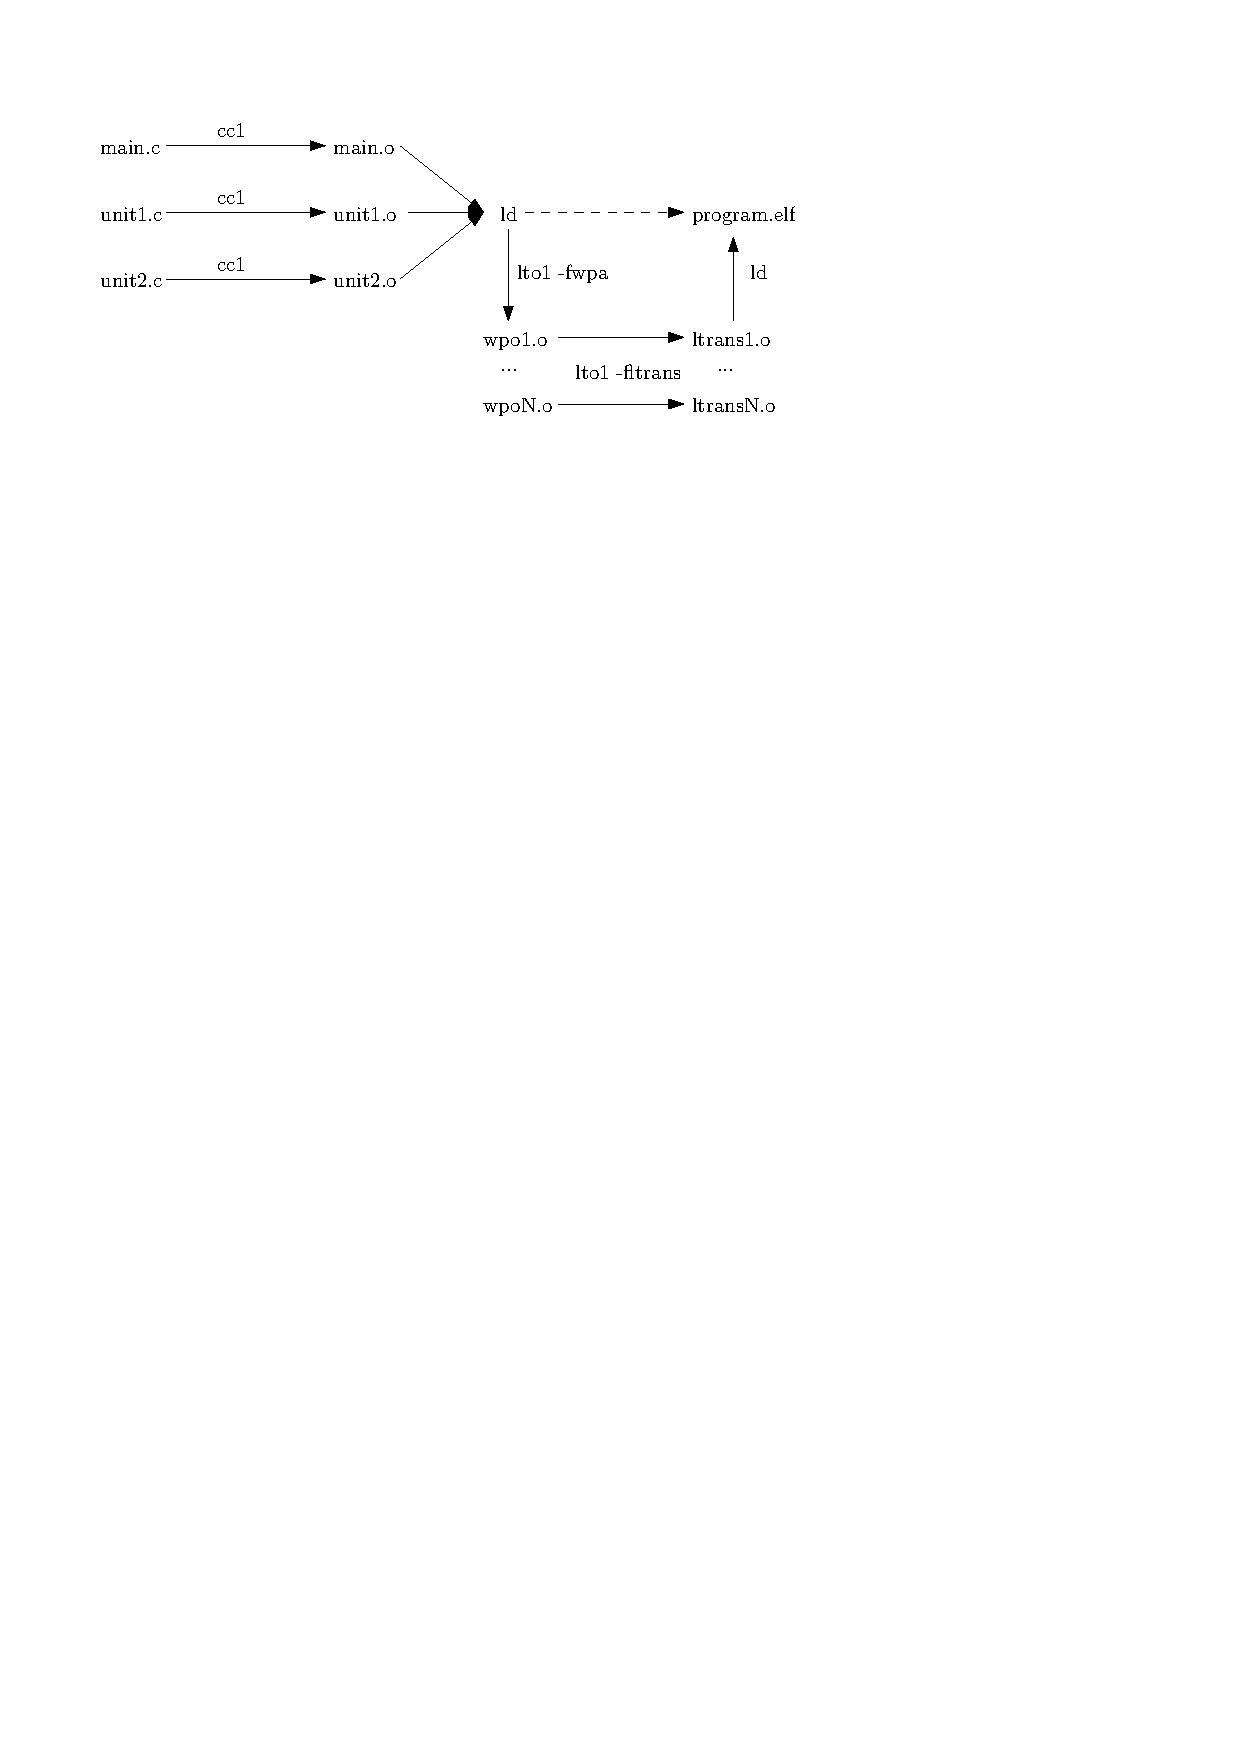
\includegraphics{./img/lto-workflow.pdf}
	\caption{Compiling source code into binary}
\end{figure}

The LTO framework (see Figure \ref{figure-lto-workflow}) solves these problems by keeping separate compilation, but
instead of generating classical object files containing machine code, the
middle end stops and writes GIMPLE representation into the object, including
some metadata (for example the call graph).

Instead of generating library, the linker then picks up the GIMPLE
representation and invokes the compiler again, to do a WPA pass. In this phase,
the object files are examined, a partial optimization plan in formed, and the
code is partitioned into smaller pieces called {\sl LTO partitions}. The
partitioning happens with regard to the code being optimized, for example to
minimize cross-partition edges.

Individual LTO partitions are then passed, separately and in parallel, to the
compiler for LTRANS\footnote{Local TRANSformations} pass. The decisions made in
WPA pass are implemented here, including additional analyses and optimizations.

The advantage of LTO partitions is that they are usually larger than original
source files and their size and content is controlled by the compiler, not by
programmers. It can also be adjusted at build time, for example it's possible
to instruct GCC to create only one LTO partition\footnote{\tt --param
lto-partitions=1}, in which case all the code is
compiled at once.


\begin{figure}[h!]
	\label{figure-firefox-ipa-kpta}
	\centering
	\includegraphics{./graphs/firefox-ipa-kpta/firefox-ipa-kpta.pdf}
	\caption{Building libxul.so with {\tt -fipa-kpta -flto=8}}
\end{figure}
